\documentclass[a4paper,12pt,twoside,openany]{article}
\usepackage{graphicx}
\usepackage{setspace}
\usepackage{listing}
\usepackage{listings}
%%\usepackage{natbibspacing}             % for bibilography 
\usepackage{bibspacing}
\usepackage{wrapfig}
\usepackage{lipsum}
\usepackage{txfonts}
\usepackage{pdfpages}
\usepackage[left=1.2in,right=0.8in]{geometry}
\graphicspath{{figures/}}
\usepackage{float}
\usepackage{caption}
\usepackage{hyperref}
\let\iint\relax
\let\iiint\relax
\let\iiiint\relax
\let\idotsint\relax
%% \usepackage{amsmath}
%% \usepackage{amssymb}
%% \usepackage{mathtools}
%% \usepackage{color}
%% \usepackage{slashed}
%% \usepackage{pdfpages}
%% \usepackage{listings}
\usepackage{siunitx}
\usepackage{latexsym}
\usepackage{enumerate}
%% \usepackage{blindtext}
\usepackage{multirow}
\usepackage{fancyhdr}
%% \usepackage[none]{hyphenat}

\pagestyle{fancy}
\fancyhf{}
\renewcommand{\headrulewidth}{0pt}
\fancyfoot[LE,RO]{(Synopsis : PHYS01201404020)}
\fancyfoot[CE,CO]{Page \thepage}

%% \newcommand*{\bfrac}[2]{\genfrac{\lbrace}{\rbrace}{0pt}{}{#1}{#2}}


\begin{document}
\begin{figure}
\centering

\includegraphics[width=0.15\linewidth]{hbnilogo.jpeg}
\end{figure}
\begin{center}
\Large{\textbf{Homi Bhabha National Institute}}\\
\normalsize{\sffamily\textbf{SYNOPSIS OF Ph. D THESIS}}\\
\ \\
\begin{tabular}{|clcp{7 cm}|}
\hline
\textbf{1.}& \textbf{Name of the student} & \textbf{:} & Suryanarayan Mondal \\[1 ex]
\textbf{2.} & \textbf{Name of the Constituent Institution} & \textbf{:} & Bhabha Atomic Research Centre, Mumbai \\[1 ex]
\textbf{3.} & \textbf{Enrolment No.} & \textbf{:} & PHYS01201404020 \\[1 ex] %(Enrollment no.)
\textbf{4.} & \textbf{Title of the Thesis} & \textbf{:} & Multiplicity of muon in $2$\,m\,$\times$\,2\,m detector and charge ratio of cosmic muon at Madurai.\\[1 ex]
\textbf{5.} & \textbf{Board of Studies} & \textbf{:} & Physical Sciences\\
\hline
\end{tabular}
\ \\
\ \vspace{12 pt}\\
{\large{\underline{\sffamily\textbf{SYNOPSIS}}}}\\
\end{center}
\doublespacing

\section{Introduction}
The 50 kton INO-ICAL\cite{inowhite} is a proposed underground high energy physics experiment at Theni, India (9$^\circ$57$'$\,N, 77$^\circ$16$'$\,E) to study the neutrino oscillation parameters using atmospheric neutrinos. The Resistive Plate Chamber (RPC) has been chosen as the active detector element for the ICAL detector, interspersed with 5.6\,cm thick iron plates. Approximately 30000 RPC gaps of dimension 2\,m\,$\times$\,2\,m will be placed in between the 151 layers of iron plates. The iron plates will be magnetised up-to about 1.5\,Tesla. The detector will be housed inside a cavern under a rock overburden of 1\,km to reduce the atmospheric muon background. The ICAL will search mainly for $\nu_{\mu}$ induced charged current interactions in the iron target. The primary aim of the experiment is to determine the sign of the mass-squared difference \mbox{$\Delta m^2_{32}$ $\left(=m^2_3-m^2_2\right)$} using matter effects. The ICAL detector can also be used to probe the value of \mbox{leptonic CP-phase $\left(\delta_{cp}\right)$} and last but not the least to search for physics beyond the standard model using neutrino oscillations. 

\section{Quality Control of RPCs}

The RPC is basically a gaseous based parallel-plate detector\cite{rpc_p2}. The RPC is constructed using two parallel plates of glass having a bulk resistivity of the order of $10^{10}$-$10^{12}$\,$\Omega$\,cm with a gas gap of a few mm. Uniform spacing between two glass plates is maintained using button spacers. Ideally, the whole chamber has to be leakproof. The outer surfaces of the glass plates are made conductive using graphite coating to form the electrodes where high voltages can be applied. The signal is readout by copper pickup strips on both sides of the RPC. In ICAL detector, the RPCs are going to be operated in avalanche mode with a gas mixture of R134a\,(95.2\%), iso-C$_4$H$_{10}$\,(4.5\%) and SF$_6$\,(0.3\%).\footnote{R134a is one of the commercial name of 1,1,1,2-Tetrafluoroethane.} R134a gas acts as a target for the ionising particles passing through the gas gap. The iso-C$_4$H$_{10}$ absorbs the photons emitted in the recombination processes limiting the formation of secondary avalanches. SF$_6$, being an electronegative gas, localizes the signal in a small area to have better position resolution.

The ICAL detector is proposed to operate for about 20 years or more. For the success of the experiment, each of the RPCs used in this experiment has to function without showing any significant ageing during the period of operation. Hence, various tests are performed during and after production. During the active operation of the ICAL detector, more than 200,000\,litres of the gas mixtures will be circulating inside the 30,000 RPCs. To achieve this, a closed-loop gas circulation system (CLS) is designed whose main purpose is to recirculate the gas mixture, minimising wastage of gas which reduces the operational cost. The leakage of the gas mixture from a closed-loop system will increase the cost of operation. Also, the leakage of outside atmosphere into the system will contaminate the gas mixture by water vapour and oxygen which may damage the RPC\cite{rpc_c,rpc_w}. The fluorine present in the RPC gas mixture will react with water vapour producing hydrofluoric acid which will damage the inner surfaces of the glass electrodes. The oxygen gas having affinity to electrons can affect the performance of the detector. Due to the aforementioned reasons, a proper leak test has to be performed on all the glass gaps at the time of production as well as during operation and a proper gas monitoring system for the CLS has to be implemented to detect impurities in the gas-mixture during operation.

\subsection{Leak Test of RPCs}
The principal aim of the current study is to test whether the RPC can hold the prescribed pressure difference or not in the presence of the variation in ambient pressure due to solar atmospheric tides.\footnote{The solar atmospheric tides are generated by the periodic heating of the atmosphere by the Sun. This regular diurnal cycle in heating generates tides in the atmosphere that have periods related to the solar day.} The detector setup and technique, described in detail in \cite{rpcleak}, not only help to determine whether the RPC is leaking or not but also allows to estimate the quantity of the leakage. As the number of the RPCs to be used in the ICAL detector is very large, the setup must be cost-effective, time-efficient and portable. The method described in this study is able to test multiple RPCs at the same time without moving them out of the storage area.

The schematics of the experimental setup is shown in Figure~\ref{fig:schematics}.
\begin{figure}
  \centering
  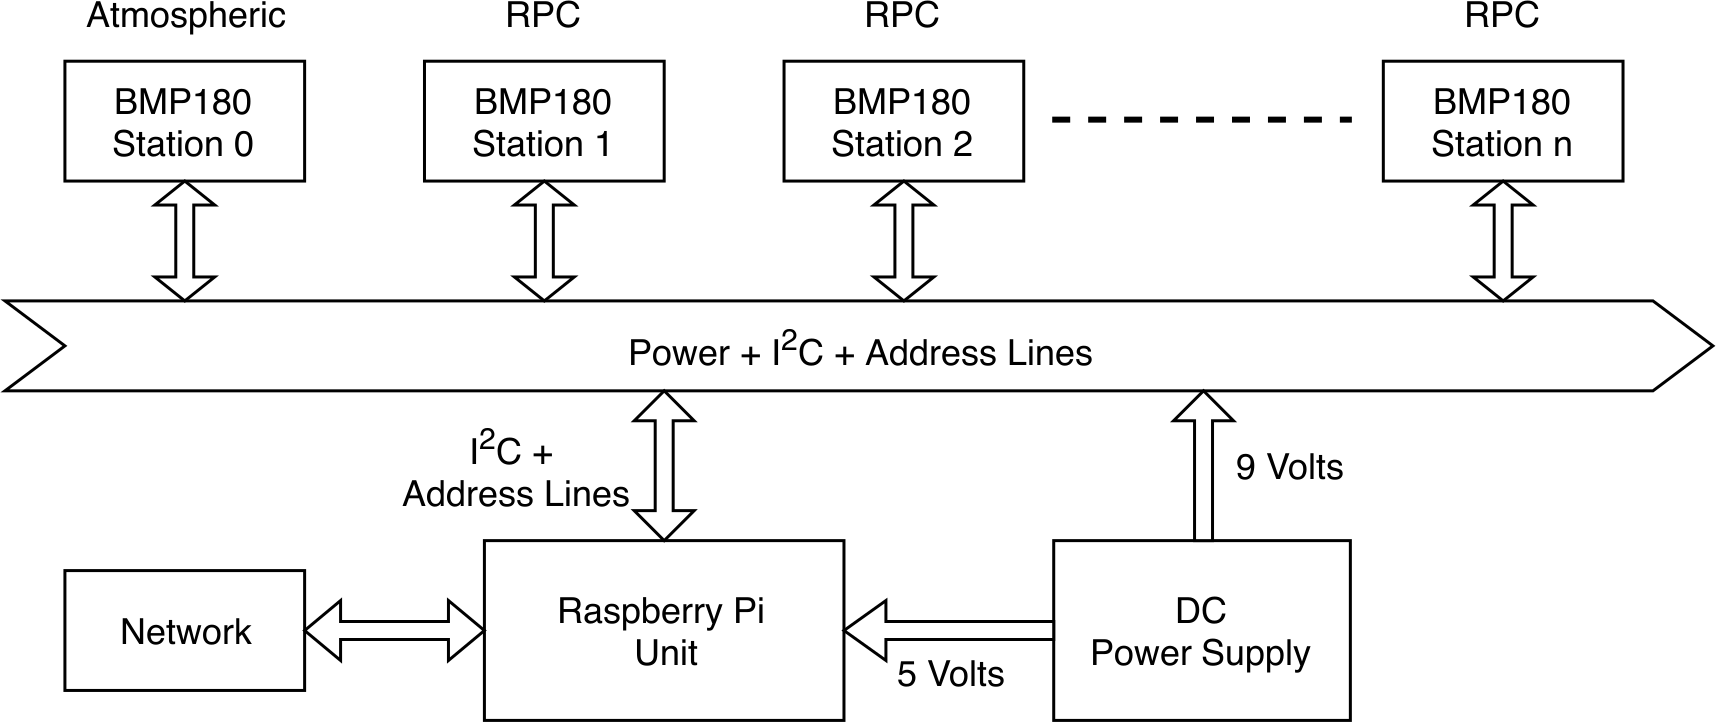
\includegraphics[width=0.9\textwidth]{leaktest_setup.png}
  \caption{Schematics of the leak test setup.}
  \label{fig:schematics}
\end{figure}
To estimate the leakage, the RPC is first pressurised up to 45\,mmWC above the atmospheric pressure and then sealed.\footnote{Millimetres water column, abbreviated to mmH$_2$O or mmWC, is a unit of pressure. It is the pressure required to support a water column of the specified height. 1\,mmWC\,$\simeq$\,0.098\,mbar.} Then the absolute pressure and temperature inside each gas gap along with the pressure and temperature of the atmosphere are measured using the sensor module, BMP180 manufactured by BOSCH\cite{bmp180}, over a long period of time. The pressure and temperature data recorded by the modules are readout over the common bus using a \textit{Raspberry Pi\,v2\,B} (Pi) unit\cite{rpi}. The data from the BMP180s can also be acquired without wires by microcontrollers equipped with WiFi modules (i.e. NodeMCU module\cite{nodemcu2015}) which utilise the WiFi network at the premises to send the data to a computer on the same network eliminating the need of the wired common bus and Pi Unit. The temperature and pressure data acquired using this system for a gas gap are shown in Figure~\ref{fig:temp}(a) and \ref{fig:temp}(b), respectively.
\begin{figure}[h!]
  \centering
  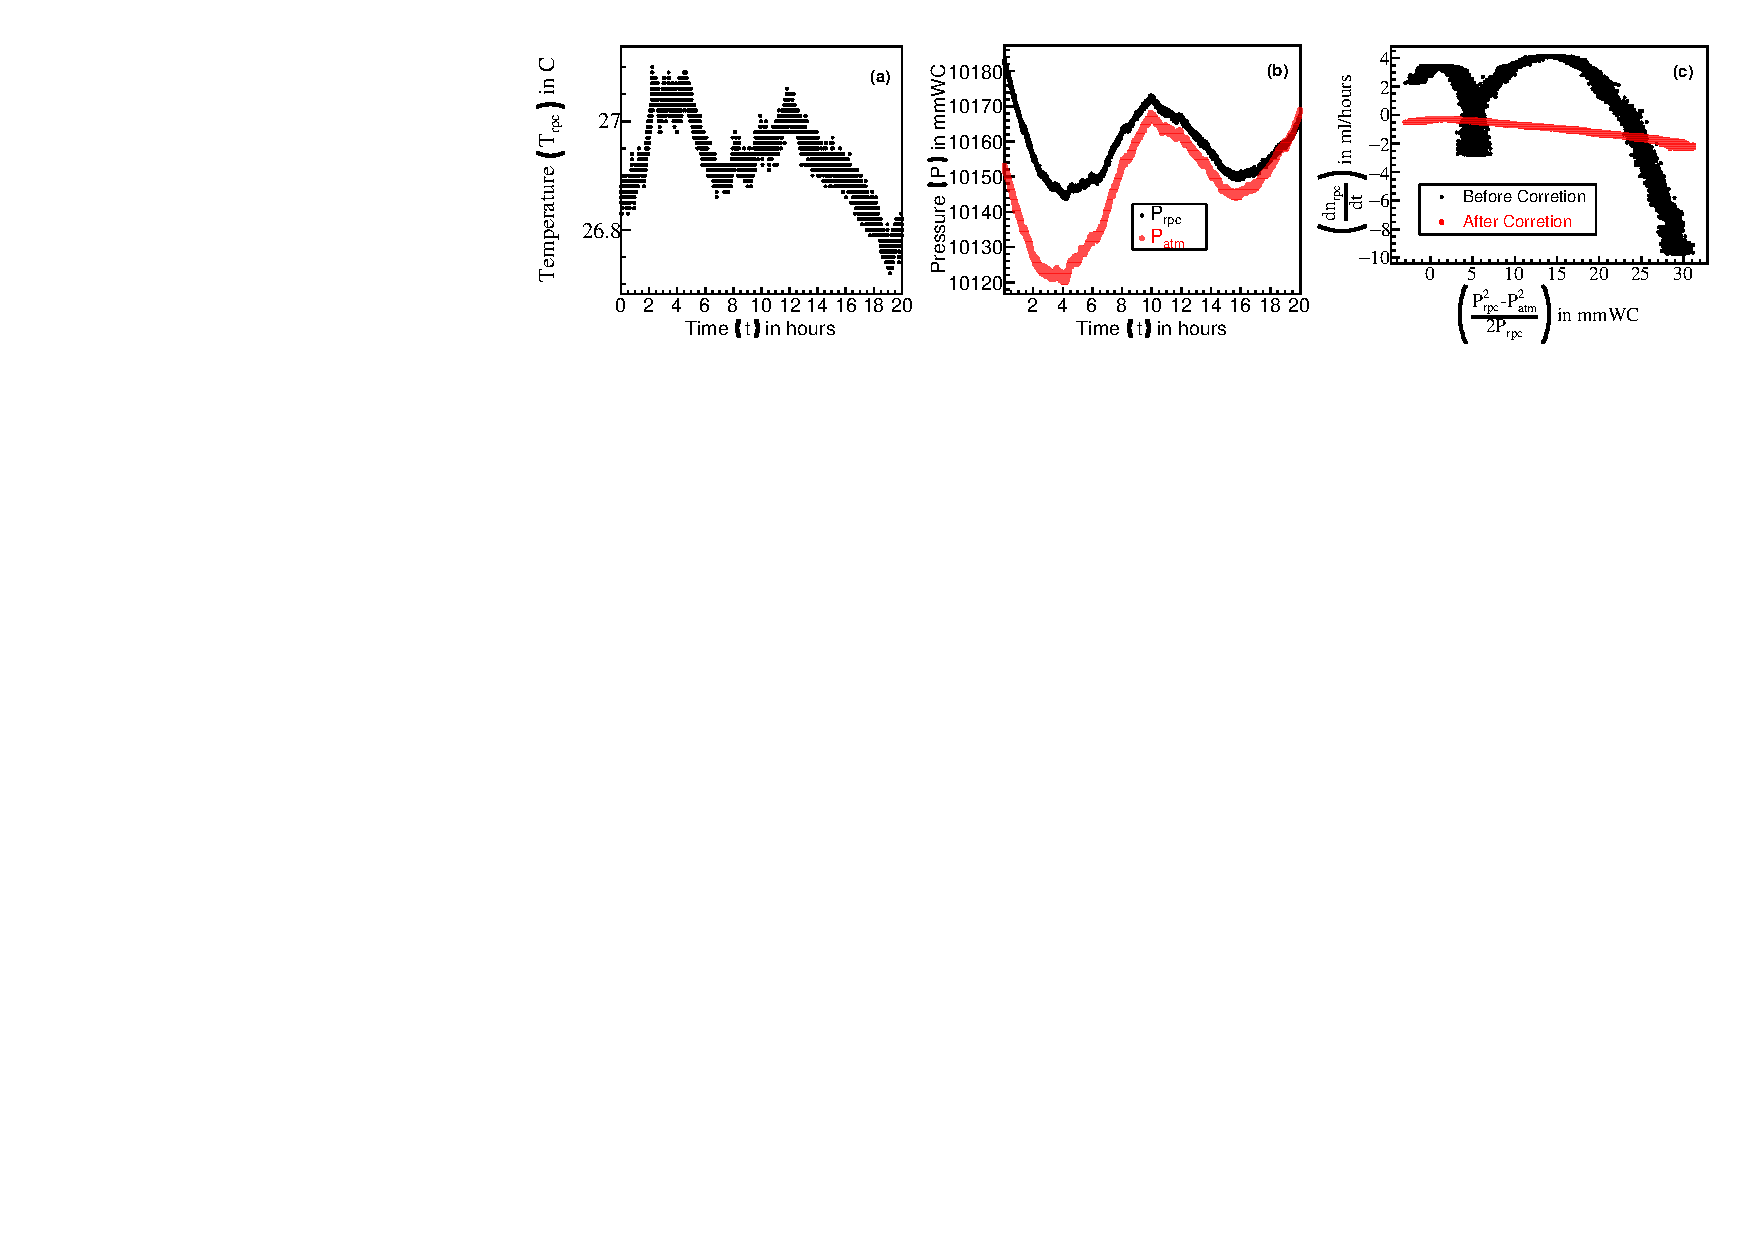
\includegraphics[width=0.99\textwidth]{all_57_3x1.pdf}
  \caption{\textbf{(a)} Variation of temperature with time, \textbf{(b)} Variation of atmospheric and RPC pressure with time, \textbf{(c)} Leak Rate vs Effective Pressure Difference plots before and after correction.}
  \label{fig:temp}
\end{figure}

The volume of the gap changes with the change of the atmospheric pressure and temperature. Assuming that the change in volume is linear to both the atmospheric pressure and the room temperature, two independent linear correction terms ($x_P$ and $x_T$) are introduced. Now, from the Ideal Gas Law, the amount of gas ($n$), inside a chamber of volume $V$, can be calculated at time $t$ using the following equation,
\begin{equation}
  n_{\textrm{rpc}\mid t}=\left(\frac{V_{\textrm{rpc}}}{R}\right)\left(\frac{P_{\textrm{rpc}\mid t}}{T_{\textrm{rpc}\mid t}}\right)\left(1-x_T\left(T_{\textrm{rpc}\mid t}-T_{\textrm{rpc}\mid t=0}\right)\right)\left(1-x_P\left(P_{\textrm{atm}\mid t}-P_{\textrm{atm}\mid t=0}\right)\right) \label{eq:ct}
\end{equation}
where, $R$ is the ideal gas constant. The leak rate at an instance during the leak test period is given by the slope of the $n$ curve. The Poiseuille's equation\cite{poiseuille} for for compressible fluids in this case is given in the following equation,
\begin{equation}
  \underbrace{\left.\frac{\mathrm{d}n_{\textrm{rpc}}}{\mathrm{d}t}\right| _t}_\text{flow/leak rate}=\underbrace{\textrm{C}_{\textrm{Leak}}}_\text{flow/leak constant}\times\underbrace{\left(\frac {P_{{\textrm{rpc}\mid t} }^{2}-P_{{\textrm{atm}\mid t} }^{2}}{2P_{{\textrm{rpc}\mid t} }}\right)}_\text{effective pressure difference}\label{eq:poiseuille}
\end{equation}
where, $\textrm{C}_{\textrm{Leak}}$ depends on the path of leakage (i.e. crack, hole, etc) and the viscosity of the gas mixture and it quantifies the leakage in the system. So, the plot of $\frac{\mathrm{d}n_{\textrm{rpc}}}{\mathrm{d}t}$ vs $\frac{P_{\textrm{rpc}}^{2}-P_{\textrm{atm}}^{2}}{2P_{\textrm{rpc}}}$ has to be a straight line if the volume is corrected properly. Best suited values of $x_T$ and $x_P$ are found for each gas gap by minimising the $\chi^2/\textrm{ndf}$ of the straight line fit of this curve. After correction, the leak rate versus the effective pressure difference is shown in Figure~\ref{fig:temp}(c) which shows a nice straight line behaviour as expected from the Poiseuille's equation. 

It should be noted that the minimal time required for a test will depend on the leakage. If the leak rate is very small then more time is needed and vice versa, but most of the gaps were able to test within 7-8 hours with a accuracy of $\sim 2\times 10^{-3}$\,ml\,hour$^{-1}$\,mmWC$^{-1}$.  Currently, a gas gap is considered as usable if its $\textrm{C}_{\textrm{Leak}}$ value is greater than $-0.02$\,ml\,hour$^{-1}$\,mmWC$^{-1}$. If the CLS is operated at an excess pressure of 10\,mmWC above atmospheric pressure, the total leakage from ICAL detector will be approximately 6\,litres/hour during its active operation.

The leak-test setups, both wired and wireless, are operational and are being used at various facilities and industries working along with INO-Collaboration and with the help of the prepared document even a novice can test a large numbers of RPCs in short time. The knowledge gained in this study also gives us more opportunity to better understand the structural integrity of the glass RPCs against various atmospheric parameters.

\section{Particle Multiplicity of Cosmic Ray Events using RPC Stack at IICHEP-Madurai}

As a part of the ICAL R\&D program, a 12 layer stack of 2\,m\,$\times$\,2\,m Resistive Plate Chambers (RPCs) with an inter-layer gap of 16\,cm has been operational at IICHEP, Madurai since last few years to study the cosmic ray muons. In the present work, the cosmic events recorded in the detector for the total observation period of $\sim$\,17\,days between August 23, 2017, to September 8, 2017, with a trigger rate of $\sim$230\,Hz are used for the analysis. The various detector properties like position and time resolution of RPCs, detector inefficiencies, strip multiplicities, detector noise, etc are studied using this RPC stack to understand the performance and long term stability of the RPCs. These observed detector parameters are included in the digitisation stage of the simulation to make it more realistic.\cite{pethu1} The data obtained by this setup is also used to study the flux and angular distribution of muons with the help of an extreme air shower (EAS) simulation program and detector simulation program. The interactions of primary cosmic ray in the air and the resultant air shower have been simulated using the CORSIKA Package\cite{corsika763}. CORSIKA is a package for detailed Monte-Carlo simulation to study the evolution of EAS in the atmosphere initiated by cosmic ray particles. The daughter particles reaching sea level in the air shower simulation in CORSIKA are given as input to the detector simulation. The detector simulation has been performed using GEANT4 toolkit\cite{geant4}. To further test the capability of the CORSIKA Package, the charged-particle multiplicity in the obtained data is compared with it with the air shower simulation.

In the CORSIKA package, the several different hadronic interaction models are available. In this study, for simulating the behaviour of hadrons for higher energy range, the QGSJET (Quark Gluon String model with JETs)\cite{corsika763} has been adopted and for the low energy range (less than 80\,GeV in laboratory frame), the GHEISHA model has been used. In this study, the primary cosmic ray shower has been simulated using the CORSIKA(v7.6300) Package. The energy of the primary rays in CORSIKA is generated using the power-law spectrum, $E^{-2.7}$, within the energy range of \mbox{$10$--$10^{6}$\,GeV} for different primaries. The zenith and azimuth angle of primary particles are generated uniformly within the range of \mbox{$0$--$85^\circ$} and \mbox{$0$--$360^\circ$}, respectively. The magnetic rigidity cutoff has been implemented according to the location of the detector site (\ang{9;56;14.5}\,N \ang{78;00;47.9}\,E, 160\,m above mean sea level). The particles generated by CORSIKA at the observation surface are provided as an input to the detector simulation. The observation plane has been divided into squares of the size of 2\,m\,$\times$\,2\,m and an event is formed using the information of the particle(s) passing through each of these rectangles shown as the shaded region in Figure~\ref{fig:eas}.
\begin{wrapfigure}{R}{0.4\linewidth}
  \centering
  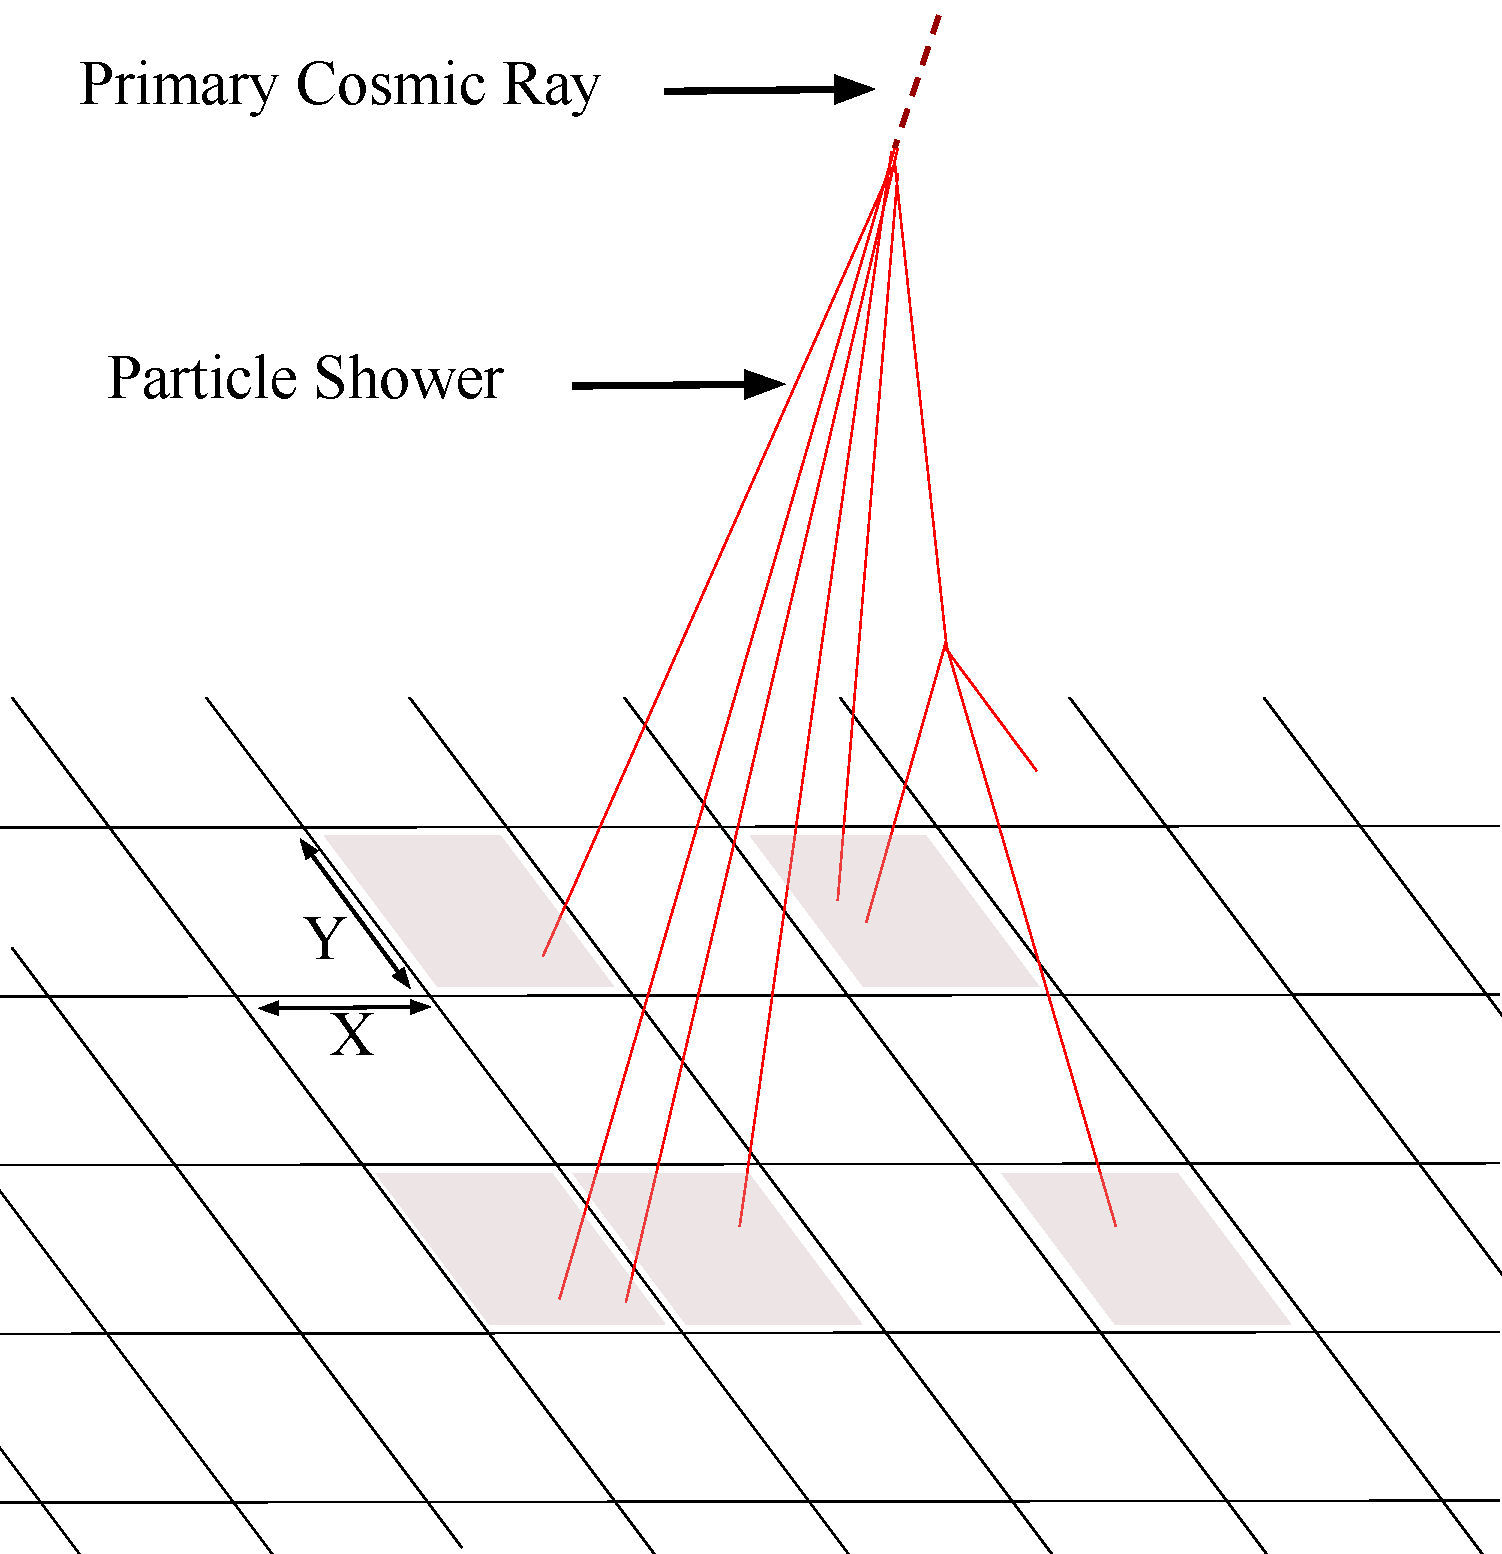
\includegraphics[width=0.99\linewidth]{EAS.pdf} 
  \caption{Shower of particles initiated by primary cosmic ray reaching observation surface.}
  \label{fig:eas}
\end{wrapfigure}

The detector simulation has been performed using GEANT4(v4-10.0.2) toolkit. The events from CORSIKA simulation are propagated in the detector simulation. A realistic depiction of the detector setup including the building where the detector is housed has been constructed in the GEANT4 environment. The properties of various materials of the detector components and the laboratory building are chosen based on the knowledge of the setup. The standard physics processes of matter-particle interactions like electromagnetic, ionisation, decay and hadronic interactions (QGSP\_BERT\_HP) are implemented in the simulation.

For the event reconstruction, the strips hits are analysed separately, in the 2-dimensional projections namely, \mbox{X--Z} and \mbox{Y--Z} plane. In the present study, the clusters are formed with a maximum of 4 consecutive strips as the position resolution for higher multiplicities is found to be worse. A layer which has more than 15 strip hits or more than 10 clusters is tagged as `noisy layer' and not considered in track reconstruction. An event which has more than 3 noisy layers is considered as `noisy event' and not used in this analysis. In the first step of track reconstruction, the clusters associated with different tracks are grouped using the method of Hough Transformation\cite{hought}. The equation of the straight line, used to find the association between the hits, is given as,
\begin{equation}
  r=z\cos\theta+x\left(/y\right)\sin\theta. \label{eq:hough}
\end{equation}

The \mbox{$r$-$\theta$} plane (called as Hough Space) is populated using the concept of Cellular Automaton\cite{cellular}. For a sample event shown in Figure~\ref{fig:houghPl}(a), the populated \mbox{$r$-$\theta$} plane is presented in Figure~\ref{fig:houghPl}(b). 
\begin{wrapfigure}{R}{0.5\textwidth}
  \centering
  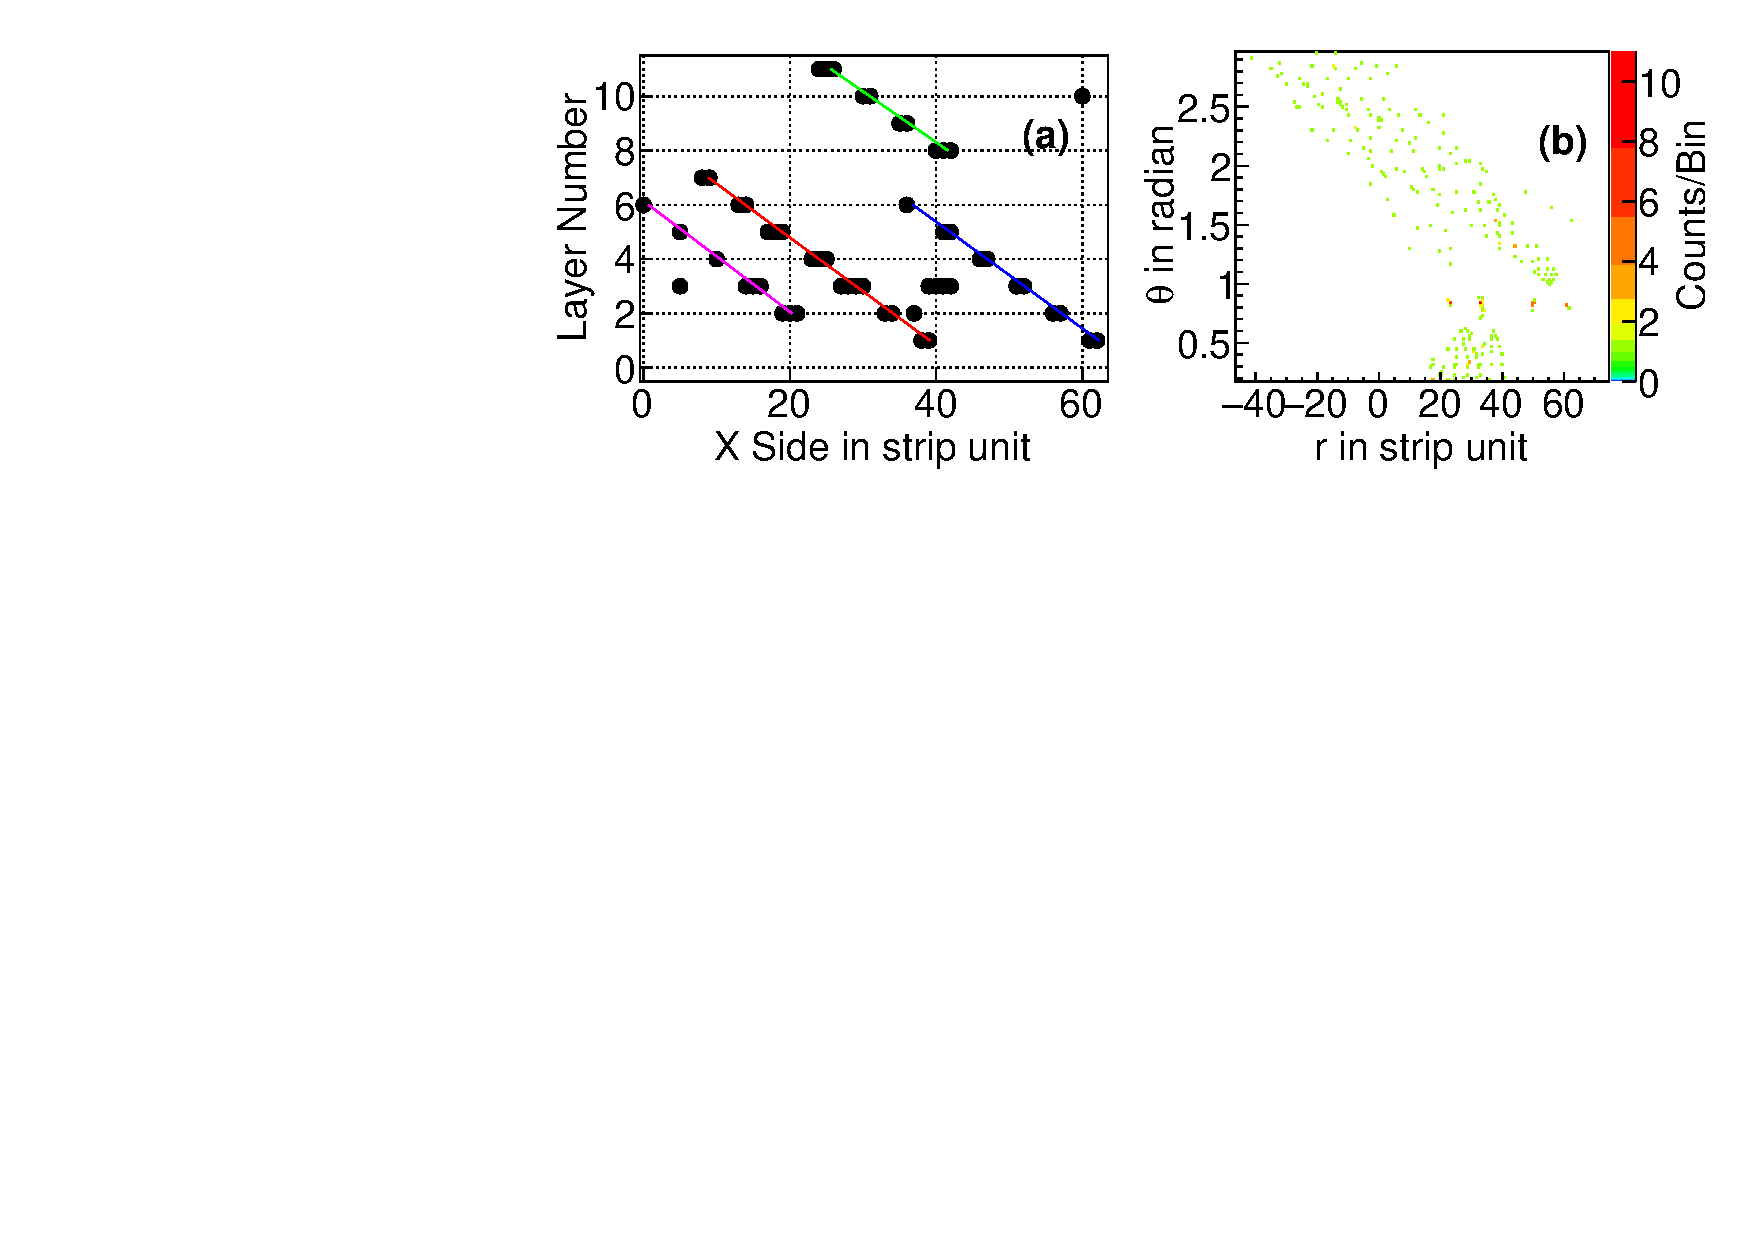
\includegraphics[width=0.99\linewidth]{hough_Plane_new.pdf} 
  \caption{(a) Projection of an event in the detector and (b) populated $r$-$\theta$~plane using this event.}
  \label{fig:houghPl}
\end{wrapfigure}
This method can detect all the tracks avoiding the noise hits as shown in Figure~\ref{fig:houghPl}(a). The projections from both X--Z and Y--Z planes are combined to produce final 3-dimensional track(s). Any ghost tracks formed while combining are discarded by using the timing information. The events of interest for this analysis are the events with more than one reconstructed 3-dimensional track. An extreme shower event (which can also be due to the noise) can imitate a multi-track event. Any such ambiguous events are rejected by the selection criteria used in the analysis.

The distribution of time separation between each pair of tracks for both simulation and data is shown in Figure~\ref{fig:time_sep}(a). In the case of data, it can be observed that there is a large number of events where multiple particles are reaching the detector with large relative time delay. The random coincidence of particles originating in the different cosmic showers is the cause for these events. In the simulation, it is observed that the particles originating from the same shower are detected in the RPC stack as parallel tracks. This can be verified by calculating the skewed angle between the two tracks which is ideally supposed to be zero in case of parallel tracks. The distribution of the skewed angle between each pair of tracks for both simulation and data is shown in Figure~\ref{fig:time_sep}(b).
\begin{figure}[h]
  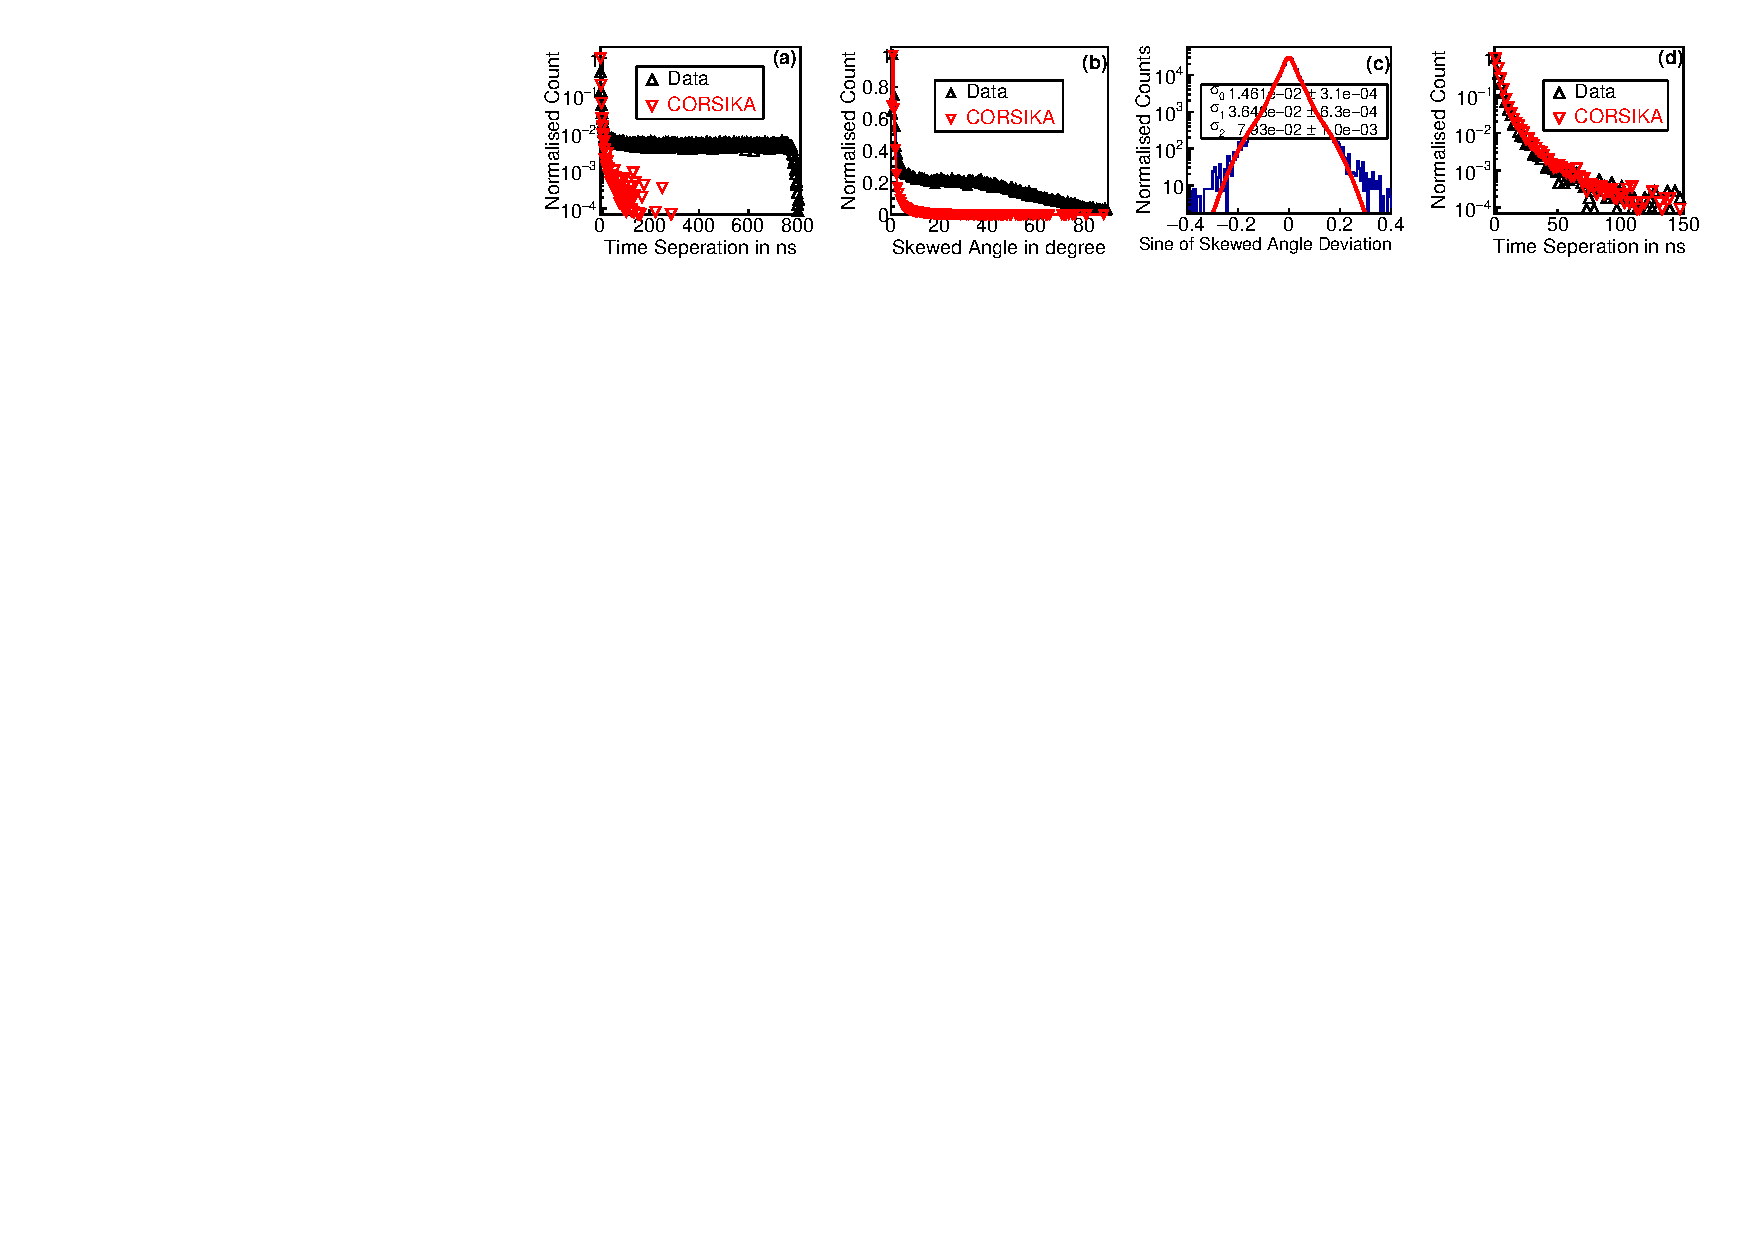
\includegraphics[width=1.0\linewidth]{time_skew_all.pdf} 
  \caption{(a) Time separation of two tracks for all events, (b) Skewed angle between two tracks originating outside of the detector, (c) Skewed angle difference between generated and reconstructed tracks fitted with triple-gaussian function and (d) Time separation of two tracks for events with only parallel tracks.}
  \label{fig:time_sep}
\end{figure}

In order to understand the application of the skewed angle, events with multiple particles are simulated in GEANT4. The distribution of the sine of the difference of the skewed angle between the generated particles and the skewed angle between the reconstructed tracks is shown in Figure~\ref{fig:time_sep}(c). This distribution is fitted with a triple-gaussian function. The three components of these angular resolutions represent the cases where; (1) no track has substantial energy loss or deviation from the original direction; (2) one track has deviated from the original direction; and (3) both the tracks have deviated from their original directions. Based on these observations, the tracks with a skewed angle less than 45\,\textit{mrad} are considered as parallel to each other. In the current study, to select the tracks generated from the particles originating from the same cosmic ray shower, only the parallel tracks are considered in the analysis. The time difference between a pair of tracks for both simulated and observed data after selecting only parallel tracks is shown in Figure~\ref{fig:time_sep}(d). It can be observed that the events from the random coincidences disappear after rejecting the events with non-parallel tracks.

The normalised fraction of events with 2, 3 and 4 tracks with respect of single track events are calculated to be \mbox{$6.35_{\pm0.05}\times 10^{-3}$\%}, \mbox{$5.8_{\pm0.5}\times 10^{-5}$\%} and \mbox{$2_{\pm1}\times 10^{-6}$\%}, respectively from the cosmic ray data. The normalised fraction of the events with 2, 3 and 4 tracks are also calculated from the CORSIKA simulation for different types of cosmic ray primaries (H, He, C, Si, and Fe) and for different hadronic interaction models (QGSJET-II-04 and QGSJET01d). In order to compare the results between the data and simulation, the normalised fractions of events are presented in Table~\ref{tab:ratio} for all different simulation scenarios mentioned above.
\begin{table}[]
  \centering
  \scalebox{0.62}{
    \begin{tabular}{cc|cccccc|c|}
\cline{3-9}
\multicolumn{1}{l}{}                                                         & \multicolumn{1}{l|}{}                                             & \multicolumn{7}{c|}{Track Fractions detected in Simulation}                                                                                                                                                                                                                                                                    \\ \cline{3-9} 
                                                                             &                                                                   & H                             & He                           & C                              & O                              & Si                             & Fe                             & \multirow{2}{*}{\begin{tabular}[c]{@{}c@{}}Combined Fractions as\\  par Abundances of \\ Cosmic Ray Particles\end{tabular}} \\ \cline{1-8}
\multicolumn{1}{|c|}{\begin{tabular}[c]{@{}c@{}}No of\\ Tracks\end{tabular}} & \begin{tabular}[c]{@{}c@{}}Track Fractions\\ in Data\end{tabular} & \multicolumn{6}{c|}{QGSJET-II-04}                                                                                                                                                                &                                                                                                                             \\ \cline{3-9} 
\multicolumn{1}{|c|}{2}                                                      & $6.35_{\pm0.05}\times 10^{-5}$                                    & $2.2_{\pm0.1}\times 10^{-5}$  & $4.7_{\pm0.2}\times 10^{-5}$ & $1.21_{\pm0.02}\times 10^{-4}$ & $1.60_{\pm0.02}\times 10^{-4}$ & $2.42_{\pm0.02}\times 10^{-4}$ & $4.58_{\pm0.03}\times 10^{-4}$ & $2.35_{\pm0.1}\times 10^{-5}$                                                                                               \\
\multicolumn{1}{|c|}{3}                                                      & $5.8_{\pm0.5}\times 10^{-7}$                                      & $1.0_{\pm0.1}\times 10^{-7}$  & $3.0_{\pm0.2}\times 10^{-7}$ & $1.78_{\pm0.05}\times 10^{-6}$ & $3.11_{\pm0.06}\times 10^{-6}$ & $5.57_{\pm0.07}\times 10^{-6}$ & $1.61_{\pm0.02}\times 10^{-5}$ & $1.2_{\pm0.1}\times 10^{-7}$                                                                                                \\
\multicolumn{1}{|c|}{4}                                                      & $2_{\pm1}\times 10^{-8}$                                          & $1.6_{\pm0.7}\times 10^{-9}$ & $9_{\pm2}\times 10^{-9}$     & $5.8_{\pm0.5}\times 10^{-8}$   & $1.12_{\pm0.07}\times 10^{-7}$ & $2.34_{\pm0.01}\times 10^{-7}$ & $1.02_{\pm0.03}\times 10^{-6}$ & $3_{\pm1}\times 10^{-9}$                                                                                                    \\ \hline
\multicolumn{1}{|c|}{\begin{tabular}[c]{@{}c@{}}No of\\ Tracks\end{tabular}} &                                                                   & \multicolumn{6}{c|}{QGSJET01d}                                                                                                                                                                   &                                                                                                                             \\ \cline{3-9} 
\multicolumn{1}{|c|}{2}                                                      &                                                                   & $2.1_{\pm0.1}\times 10^{-5}$  & $4.7_{\pm0.1}\times 10^{-5}$ & $1.18_{\pm0.02}\times 10^{-4}$ & $1.51_{\pm0.02}\times 10^{-4}$ & $2.50_{\pm0.02}\times 10^{-4}$ & $4.56_{\pm0.03}\times 10^{-4}$ & $2.36_{\pm0.1}\times 10^{-5}$                                                                                               \\
\multicolumn{1}{|c|}{3}                                                      &                                                                   & $9_{\pm1}\times 10^{-8}$      & $3.9_{\pm0.2}\times 10^{-7}$ & $1.90_{\pm0.04}\times 10^{-6}$ & $3.14_{\pm0.08}\times 10^{-6}$ & $6.19_{\pm0.07}\times 10^{-6}$ & $1.65_{\pm0.02}\times 10^{-5}$ & $1.2_{\pm0.1}\times 10^{-7}$                                                                                                \\
\multicolumn{1}{|c|}{4}                                                      &                                                                   & $8_{\pm4}\times 10^{-10}$     & $7_{\pm1}\times 10^{-9}$     & $6.0_{\pm0.4}\times 10^{-8}$   & $1.07_{\pm0.07}\times 10^{-7}$ & $3.4_{\pm0.1}\times 10^{-7}$   & $1.6_{\pm0.03}\times 10^{-6}$  & $2.4_{\pm0.6}\times 10^{-9}$                                                                                                \\ \hline
\end{tabular}}
  \caption{Amount of track fraction with 2, 3 and 4 tracks obtained from Simulation compared to that of Data for different primaries (H, He, C, O, Si and Fe) and different physics packages (QGSJET-II-04 and QGSJET01d).}\label{tab:ratio}
\end{table}

If the abundances of elements in primary cosmic ray spectrum as observed in \cite{cosmic1} are used to form the final result from simulation, the normalized track fraction with 2, 3 and 4 tracks are $2.35_{\pm0.1}\times 10^{-5}$, $1.2_{\pm0.1}\times 10^{-7}$ and $3_{\pm1}\times 10^{-9}$ for the QGSJET-II-4 model and $2.36_{\pm0.1}\times 10^{-5}$, $1.2_{\pm0.1}\times 10^{-7}$ and $2.4_{\pm0.6}\times 10^{-9}$ for the QGSJET01d model, respectively.

The results of the current study reflect that the current physics models of interactions at the earth atmosphere are unable to reproduce the air showers accurately. The earlier measurements of muon multiplicity (KGF\cite{kgf1}, ALICE\cite{alice1}, MACRO\cite{macro1}, DELPHI\cite{delphi1}, ALEPH\cite{aleph1} and KASCADE-Grande\cite{kascade1}) which also showed more muon multiplicity in data along with the present result can be used to improve the parameters of the hadronic model at high energies and/or cosmic ray spectral index.

\section{Charge Ratio of Atmospheric Muons at IICHEP-Madurai}

As a part of the ICAL R\&D program, a magnetised detector (mini-ICAL) with 10 layers of RPCs has been operational at IICHEP, Madurai to study the performance of electronics equipment in the presence of magnetic field and to test the event reconstruction algorithms. One of the motivations of the magnetised mini-ICAL detector was to estimate the muon charge ratio at Madurai and compare the result with CORSIKA simulation which is very near to the INO site. The muon charge ratio $R$ is defined as the ratio of $\mu+$ to $\mu-$ arriving at the Earth's surface. These muons are created at the upper atmosphere due to the interaction of the high energetic primary cosmic rays and the air molecules. As the primary cosmic rays are dominated by the positively charged particles, the production of the positive mesons are favoured. Measurement of the muon charge ratio can be used to improve the hadronic interaction models and for better neutrino flux prediction.

The mini-ICAL detector operational at IICHEP, Madurai is consist of 11 layers of iron of size 4\,m\,$\times$\,4\,m\,$\times$\,5.6\,cm with the interlayer gap of 4.5\,cm. A uniform magnetic field of 1.3\,T is obtained in the central region of the detector by winding the copper conductors in a similar fashion to the proposed ICAL detector. The magnetic field in the mini-ICAL is along the Y-direction in the central region. Ten RPCs of dimensions 174\,cm\,$\times$\,183.5\,cm are used as the active detector. These RPCs are and placed in the central region of the detector in between iron layers. The DAQ system is similar to the setup discussed previously.

The reconstruction of momentum and charge of muons has been performed in two stages. At first, an event is fitted with the equation of a circle. The charge, rough momentum and initial direction of the muon are estimated by observing the curvature of the fitted circle. This information is then used in the second stage as input parameters. In the second stage, the muon is then propagated in the detector medium including ionisation energy loss in iron and other material.

The result of this study will be used to improve the hadronic interaction models and for better prediction of neutrino flux.

\section{Summary}
The RPCs in ICAL detector is proposed to operate for 20 years. For the success of the experiment, each of the RPCs used in this experiment has to function without showing any significant ageing during the period of operation. Hence, a proper leak test has to be performed on all the glass gaps at the time of production as well as during operation and a proper gas monitoring system for the CLS has to be implemented to detect impurities in the gas-mixture during operation which can be included in ICAL detector with very low cost.

The method of testing gaps for leakage and quantifying the leak is developed. The leak-test setups, both wired and wireless, are operational and are being used at various facilities and industries working along with INO-Collaboration. The test setups have decreased the average time required per gap significantly. The knowledge gained in this study also gives us more opportunity to better understand the structural integrity of the glass RPCs against various atmospheric parameters. An FTIR setup in the spectral range of \mbox{2-20\,$\mu$m} and with a spectral resolution of \mbox{$\sim$0.05\,cm$^{-1}$} is in development to detect all the gases and impurity fractions in the gas mixture during the operation.

As a part of the ICAL R\&D program, a 12 layer stack of 2\,m\,$\times$\,2\,m Resistive Plate Chambers (RPCs) has been operational at IICHEP, Madurai since last few years to study the various detector properties. The cosmic ray data acquired at this stack is studied for charged-particle multiplicity. The charged-particle multiplicity in the obtained data is compared with the air shower simulation. The main aim of this study is to test the capability of the cosmic ray simulation packages. It reflects that the current physics models of interactions at the earth atmosphere are unable to reproduce the air showers accurately. The earlier measurements of muon multiplicity which have similar conclusions along with the present result can be used to improve the parameters of the hadronic model at high energies and/or cosmic ray spectral index.

A magnetised detector (mini-ICAL) with 10 layers of RPCs also has been operational at IICHEP, Madurai to study the performance of electronics equipment in the presence of magnetic field and to test the event reconstruction algorithms. One of the motivations of the magnetised mini-ICAL detector was to estimate the muon charge ratio at Madurai and compare the result with simulation which is very near to the INO site. The result of this study can also be used to improve the hadronic interaction models and for better neutrino flux prediction. This study will also intend to improve the charge and momentum sensitivity in the ICAL detector.


\begin{thebibliography}{9}

\bibitem{inowhite}
  ICAL Collaboration,  \emph{Invited review: Physics potential of the ICAL Detector at the India-based Neutrino Observatory (INO)}, \emph{Pramana J. Phys., Volume } \textbf{88(5)}, 79 (Apr 2017)
  
%% \bibitem{rpc_p1}
%%   Pestov, {\relax Yu}. N. and Fedotovich, G. V., \emph{A PICOSECOND TIME-OF-FLIGHT SPECTROMETER FOR THE VEPP-2M BASED ON LOCAL -  DISCHARGE SPARK COUNTER}, \emph{SLAC-TRANS-0184, IYF-77-78} (1978)
  
\bibitem{rpc_p2}
  R.~Santonico and R.~Cardarelli, \emph{Development of resistive plate counters}, \emph{Nuclear Instruments and Methods in Physics Research, Volume} \textbf{187} (1981) 377-380

\bibitem{rpc_c}
  S.~Colafranceschi~et.~al. \emph{A study of gas contaminants and interaction with materials in rpc closed loop systems}, \emph{Journal Of Instrumentation, Volume } \textbf{8(03)}, T03008 (2013)

\bibitem{rpc_w}
  H.~Sakai~et.~al. \emph{Study of the Effect of Water Vapor on a Resistive Plate Chamber with Glass Electrodes}, \emph{Nuclear Instruments and Methods in Physics Research Section A: Accelerators, Spectrometers, Detectors and Associated Equipment, Volume } \textbf{484(1-3)}, 153--161 (2002)

\bibitem{rpcleak}
  S.~Mondal~et.~al. \emph{Leak test of Resistive Plate Chamber gap by monitoring absolute pressure}, \href{https://doi.org/10.1088/1748-0221/14/04/P04009}{\emph{Journal of Instrumentation, Volume } \textbf{14}, P04009 (April 2019)}

\bibitem{bmp180}
  Bosch Sensortec, \emph{Digital Pressure Sensor}, \emph{May} 7$^\mathrm{th}$ 2015 [\emph{Revision} \textbf{2.8}]

\bibitem{rpi}
  \emph{Raspberry Pi 2 Model B}, \emph{https://www.raspberrypi.org/products/raspberry-pi-2-model-b/} dated 23rd Nov 2018
    
\bibitem{nodemcu2015}
  Agus Kurniawan, \emph{NodeMCU Development Workshop}, PE Press (July 2015)

\bibitem{poiseuille}
  J.~Pfitzner, \emph{Poiseuille and his law}, \emph{Anaesthesia, Volume } \textbf{31}, 273-275 (1976)
  
  
\bibitem{pethu1}
  S.~Pethuraj~et.~al., \emph{Measurement of cosmic muon angular distribution and vertical integrated flux by 2\,m$\times$2\,m {RPC} stack at {IICHEP}-Madurai}, \href{https://doi.org/10.1088/1475-7516/2017/09/021}{\emph{Journal of Cosmology and Astroparticle Physics, Vol} \textbf{09}, 021-021 (2017)}
  
\bibitem{corsika763}
  D.~Heck~et.~al. \emph{1998 CORSIKA: A Monte Carlo Code to Simulate Extensive Air Showers}, \href{https://www.ikp.kit.edu/corsika/70.php}{Forschungszentrum Karlsruhe Report FZKA 6019}
    
\bibitem{geant4}
  GEANT4 collaboration, S.~Agostinelli~et~al., \textit{GEANT4: A Simulation toolkit}, \href{https://doi.org/10.1016/j.nima.2010.08.075}{Nucl. Instrum.  Meth. A 506 (2003) 250 [ IN SPIRE ]}.
  
%% \bibitem{nino}
%%   F.~Anghinolfi~et~al., \emph{NINO: an ultra-fast and low-poer front-end amplifier/discriminator ASIC designed for the multigap resistive plate chamber}, \emph{Nucl. Instrum. Methods A} {\bf 533} (2004) 183-187.

%% \bibitem{anusp}
%%   V.~B.~Chandratre, Menka~Sukhwani, K~Hari~Prasad, Sourav~Mukhopadhyay, Megha~Thomas, Ravindra~Shinde and Satyanarayana~B., \emph{ANUSPARSH-II frontend ASIC for avalanche mode of RPC detector using regulated cascode trans-impedance amplifier}, \emph{Proceedings of the DAE-BRNS Symp. on Nucl. Phys., Vol} {\bf 60} (2015) 928-929.

\bibitem{elec1}
  Achrekar~S.~et~al. \emph{Electronics, Trigger and Data Acquisition Systems for the INO ICAL Experiment. In: Liu ZA. (eds) Proceedings of International Conference on Technology and Instrumentation in Particle Physics 2017. TIPP 2017. Springer Proceedings in Physics, vol 212. Springer, Singapore} (2018)

\bibitem{hought}
  Niu~Li-Bo~et.~al. \emph{Track reconstruction based on Hough-transform for nTPC}, \emph{Chinese Physics C, Vol} 38(12) 126201
  
\bibitem{cellular}
  Zhaoyi~Qu~et.~al. \emph{New track finding based on cellar automaton for AMS-02 detector}, \emph{Nuclear Instruments and Methods in Physics Research Section A, Vol} 869 (11 Oct 2017) 135-140
  
\bibitem{cosmic1}
  M.~M.~Shapiro~et.~al. \emph{Relative Abundances of Cosmic Rays at their Source (Proceedings of 11$^{th}$ International Conference on Cosmic Rays, Budapest 1969)}, \emph{Acta Physica Academiae Scientiarum Hungaricae}, \textbf{29} Suppl. 1 (1970) 479-484 

\bibitem{kgf1}
  H.~Adarkar~et.~al., \emph{A multi TeV muon bundle observed in the KGF underground detector}, \emph{Physics Letters B, Vol} \textbf{267}(1) (September 1991) 138-142 [\href{https://doi.org/10.1016/0370-2693(91)90539-3}{10.1016/0370-2693(91)90539-3}]

\bibitem{alice1}
  The~ALICE~Collaboration, \emph{Study of cosmic ray events with high muon multiplicity using the ALICE detector at the CERN Large Hadron Collider}, \emph{Journal of Cosmology and Astroparticle Physics, Vol} \textbf{2016} (January 2016) 032 [\href{https://doi.org/10.1088/1475-7516/2016/01/032}{10.1088/1475-7516/2016/01/032}]

\bibitem{macro1}
  The~MACRO~Collaboration, \emph{Multiple Muon Measurements with MACRO}, \emph{Proceedings, Very High Energy Cosmic Ray Interactions,} \textbf{C94-07-24} (1994) 711-722 [\href{https://arxiv.org/abs/hep-ex/9410001}{hep-ex/9410001}]

\bibitem{delphi1}
  The~DELPHI~Collaboration, \emph{Study of multi-muon bundles in cosmic ray showers detected with the DELPHI detector at LEP}, \emph{Astroparticle Physics, Volume }\textbf{28}(3) (November 2007) 273-286 [\href{https://doi.org/10.1016/j.astropartphys.2007.06.001}{10.1016/j.astropartphys.2007.06.001}]

\bibitem{aleph1}
  V.~Avati~et.~al., \emph{Cosmic multi-muon events observed in the underground CERN-LEP tunnel with the ALEPH experiment}, \emph{Astroparticle Physics, Volume }\textbf{19}(3) (November 2002) 513¡V523 [\href{https://doi.org/10.1016/S0927-6505(02)00247-5}{10.1016/S0927-6505(02)00247-5}]

\bibitem{kascade1}
  W.~D.~Apel~et.~al., \emph{Probing the evolution of the EAS muon content in the atmosphere with KASCADE-Grande}, \emph{Astroparticle Physics, Volume }\textbf{95} (2017) 25¡V43 [\href{https://doi.org/10.1016/j.astropartphys.2017.07.001}{10.1016/j.astropartphys.2017.07.001}]

\end{thebibliography}



%% \cleardoublepage

%% Publications in Refereed Journal:
%% a. Published
%% b. Accepted:
%% c. Communicated:
%% Other Publications:
%% a. Book/Book Chapter
%% b. Conference/Symposium
%% Signature of Student:
%% Date:

\clearpage{\thispagestyle{empty}\cleardoublepage}

\noindent\textbf{Publications in Refereed Journal:}
\begin{enumerate}[a.]
\item Published:
  \begin{enumerate}[1)]
  \item \textbf{S.~Mondal}, V.~M.~Datar, S.~D.~Kalmani, G.~Majumder, N.~K.~Mondal, K.~C.~Ravindran and B.~Satyanarayana, \emph{Leak test of Resistive Plate Chamber gap by monitoring absolute pressure}, \href{https://doi.org/10.1088/1748-0221/14/04/P04009}{\emph{Journal of Instrumentation, Volume } \textbf{14} (April 2019) P04009}
  \end{enumerate}
%% \item Accepted:
\item Communicated:
  \begin{enumerate}[1)]
  \item \textbf{S.~Mondal}, V.~M.~Datar, S.~D.~Kalmani, G.~Majumder, N.~K.~Mondal, S.~Pethuraj, K.~C.~Ravindran and B.~Satyanarayana, \emph{Study of Particle Multiplicity of Cosmic Ray Events using 2\,m\,$\times$\,2\,m Resistive Plate Chamber Stack at IICHEP-Madurai}, \emph{Experimental Astronomy}, \textbf{EXPA-D-19-00048R1}, \href{https://arxiv.org/abs/1908.04589}{arXiv:1908.04589}
  \end{enumerate}
\end{enumerate}

\noindent\textbf{Other Publications:}
\begin{enumerate}[a.]
\item Conference/Symposium
  \begin{enumerate}[1)]
  \item \textbf{S.~Mondal}, V.~M.~Datar, S.~D.~Kalmani, G.~Majumder, N.~K.~Mondal and B.~Satyanarayana, \emph{Leak Rate Estimation of a Resistive Plate Chamber Gap by Monitoring Absolute Pressure in 13th Workshop on Resistive Plate Chambers and Related Detectors (RPC2016)}, \href{https://doi.org/10.1088/1748-0221/11/11/C11009}{\emph{Journal of Instrumentation, Volume } \textbf{11} (Nov 2016) C11009}
  \item \textbf{S.~Mondal}, V.~M.~Datar, S.~D.~Kalmani, G.~Majumder, N.~K.~Mondal and B.~Satyanarayana, \emph{Estimation of Leak of a Resistive Plate Chamber by Monitoring Absolute Pressure in XXII DAE High Energy Physics Symposium}, \href{https://doi.org/10.1007/978-3-319-73171-1_207}{\emph{Springer Proceedings in Physics, Volume } \textbf{203} (May 2018) 851-853}
  \item Gobinda~Majumder and \textbf{Suryanaraya~Mondal}, \emph{Design, construction and performance of magnetised mini-ICAL detector module in The 39th International Conference on High Energy Physics (ICHEP2018)}, \href{https://doi.org/10.22323/1.340.0360}{\emph{Proceedings of Science,} \textit{Volume} \textbf{340} (2019) 360}
  \item S.~Pethuraj, V.~M.~Datar, S.~D.~Kalmani, G.~Majumder, N.~K.~Mondal, \textbf{S.~Mondal}, P.~Nagaraj, Pathaleswar, K.~C.~Ravindran, M.~N.~Saraf, B.~Satyanarayana, R.~R.~Shinde, Dipankar~Sil, S.~H.~Thoker, S.~S.~Upadhya, P.~Verma and E.~Yuvaraj, \emph{Measurement of Angular Distribution and Integrated Flux of Cosmic Ray Muons Using 2\,m$\times$2\,m RPC Stack at IICHEP Madurai in XXII DAE High Energy Physics Symposium}, \href{https://doi.org/10.1007/978-3-319-73171-1_205}{\emph{Springer Proceedings in Physics,} \emph{Volume} \textbf{203} (2018) 845-846}
  \item G.~Majumder, V.~M.~Datar, S.~D.~Kalmani, N.~K.~Mondal, \textbf{S.~Mondal}, B.~Satyanarayana and R.~R.~Shinde, \emph{Development of a Resistive Plate Chamber with Heat Strengthened Glass in XXII DAE High Energy Physics Symposium}, \href{https://doi.org/10.1007/978-3-319-73171-1_135}{\emph{Springer Proceedings in Physics, Volume} \textbf{203} (2018) 575-578}
  \item  G.~Majumder, V.~M.~Datar, S.~D.~Kalmani, N.~K.~Mondal, \textbf{S.~Mondal}, B.~Satyanarayana and R.~R.~Shinde, \emph{Development of a Resistive Plate Chamber with heat strengthened glass in 13th Workshop on Resistive Plate Chambers and Related Detectors (RPC2016)}, \href{https://doi.org/10.1088/1748-0221/11/09/C09019}{\emph{Journal of Instrumentation, Volume} \textbf{11} (2016) C09019}
    \item S.~D.~Kalmani, \textbf{S.~Mondal}, R.~R.~Shinde and P.~V.~Hunagund, \emph{Some Studies Using Capillary for Flow Control in a Closed Loop Gas Recirculation System in XXII DAE High Energy Physics Symposium}, \href{https://doi.org/10.1007/978-3-319-73171-1_223}{\emph{Springer Proceedings in Physic, Volume} \textbf{203} (2018) 913-915}
  \end{enumerate}
\end{enumerate}

\vskip 3em

\hspace*{1em}{\rm Suryanarayan Mondal}\\
\hspace*{2.5em}{\rm (Enrolment Number: PHYS01201404020)}


\newpage
\singlespacing
\noindent\textbf{Doctoral Committee}
\begin{center}
\begin{tabular}{|c|p{6 cm}|c|l|c|}
\hline
\textbf{S. No}& \textbf{Name} & \textbf{Designation} & \textbf{Signature} & \textbf{Date} \\
\hline
1. & Amol Dighe & Chairman&\hspace{3 cm} &\hspace{1.7 cm} \\
&  & & & \\
\hline
2. &  Prashant Shukla & Guide/ & & \\
& & Convener & & \\
\hline
3. & Gobinda Majumder & Co-guide & & \\
& & & & \\
\hline
4. & Subhasish Chattopadhyay & Member& & \\
 & & & & \\
\hline
5. & Supratik Mukhopadhyay & Member & & \\
 &  & & & \\
\hline
\end{tabular}
\end{center}
\ \\
\ \\
\ \\
\ \\
\begin{flushright}
  \textbf{Dean-Academic, CI}\\
\end{flushright}
\ \\
\ \\
\ \\
\ \\
\textbf{To} \\
\textbf{Dean, HBNI}

\end{document}
